\documentclass[,man,floatsintext]{apa6}
\usepackage{lmodern}
\usepackage{amssymb,amsmath}
\usepackage{ifxetex,ifluatex}
\usepackage{fixltx2e} % provides \textsubscript
\ifnum 0\ifxetex 1\fi\ifluatex 1\fi=0 % if pdftex
  \usepackage[T1]{fontenc}
  \usepackage[utf8]{inputenc}
\else % if luatex or xelatex
  \ifxetex
    \usepackage{mathspec}
  \else
    \usepackage{fontspec}
  \fi
  \defaultfontfeatures{Ligatures=TeX,Scale=MatchLowercase}
\fi
% use upquote if available, for straight quotes in verbatim environments
\IfFileExists{upquote.sty}{\usepackage{upquote}}{}
% use microtype if available
\IfFileExists{microtype.sty}{%
\usepackage{microtype}
\UseMicrotypeSet[protrusion]{basicmath} % disable protrusion for tt fonts
}{}
\usepackage{hyperref}
\hypersetup{unicode=true,
            pdftitle={Early language experience in a Papuan village},
            pdfauthor={Marisa Casillas, Penelope Brown, \& Stephen C. Levinson},
            pdfkeywords={Child-directed speech, linguistic input, non-WEIRD, vocal maturity,
interaction, Papuan},
            pdfborder={0 0 0},
            breaklinks=true}
\urlstyle{same}  % don't use monospace font for urls
\usepackage{graphicx}
% grffile has become a legacy package: https://ctan.org/pkg/grffile
\IfFileExists{grffile.sty}{%
\usepackage{grffile}
}{}
\makeatletter
\def\maxwidth{\ifdim\Gin@nat@width>\linewidth\linewidth\else\Gin@nat@width\fi}
\def\maxheight{\ifdim\Gin@nat@height>\textheight\textheight\else\Gin@nat@height\fi}
\makeatother
% Scale images if necessary, so that they will not overflow the page
% margins by default, and it is still possible to overwrite the defaults
% using explicit options in \includegraphics[width, height, ...]{}
\setkeys{Gin}{width=\maxwidth,height=\maxheight,keepaspectratio}
\IfFileExists{parskip.sty}{%
\usepackage{parskip}
}{% else
\setlength{\parindent}{0pt}
\setlength{\parskip}{6pt plus 2pt minus 1pt}
}
\setlength{\emergencystretch}{3em}  % prevent overfull lines
\providecommand{\tightlist}{%
  \setlength{\itemsep}{0pt}\setlength{\parskip}{0pt}}
\setcounter{secnumdepth}{0}
% Redefines (sub)paragraphs to behave more like sections
\ifx\paragraph\undefined\else
\let\oldparagraph\paragraph
\renewcommand{\paragraph}[1]{\oldparagraph{#1}\mbox{}}
\fi
\ifx\subparagraph\undefined\else
\let\oldsubparagraph\subparagraph
\renewcommand{\subparagraph}[1]{\oldsubparagraph{#1}\mbox{}}
\fi

%%% Use protect on footnotes to avoid problems with footnotes in titles
\let\rmarkdownfootnote\footnote%
\def\footnote{\protect\rmarkdownfootnote}


  \title{Early language experience in a Papuan village}
    \author{Marisa Casillas\textsuperscript{1}, Penelope Brown\textsuperscript{1},
\& Stephen C. Levinson\textsuperscript{1}}
    \date{}
  
\shorttitle{Early language experience in a Papuan village}
\affiliation{
\vspace{0.5cm}
\textsuperscript{1} Max Planck Institute for Psycholinguistics}
\keywords{Child-directed speech, linguistic input, non-WEIRD, vocal maturity, interaction, Papuan\newline\indent Word count: XXXXX (XXXX not including references)}
\usepackage{csquotes}
\usepackage{upgreek}
\captionsetup{font=singlespacing,justification=justified}

\usepackage{longtable}
\usepackage{lscape}
\usepackage{multirow}
\usepackage{tabularx}
\usepackage[flushleft]{threeparttable}
\usepackage{threeparttablex}

\newenvironment{lltable}{\begin{landscape}\begin{center}\begin{ThreePartTable}}{\end{ThreePartTable}\end{center}\end{landscape}}

\makeatletter
\newcommand\LastLTentrywidth{1em}
\newlength\longtablewidth
\setlength{\longtablewidth}{1in}
\newcommand{\getlongtablewidth}{\begingroup \ifcsname LT@\roman{LT@tables}\endcsname \global\longtablewidth=0pt \renewcommand{\LT@entry}[2]{\global\advance\longtablewidth by ##2\relax\gdef\LastLTentrywidth{##2}}\@nameuse{LT@\roman{LT@tables}} \fi \endgroup}


\usepackage{lineno}

\linenumbers

\authornote{

Correspondence concerning this article should be addressed to Marisa
Casillas, P.O. Box 310, 6500 AH Nijmegen, The Netherlands. E-mail:
\href{mailto:Marisa.Casillas@mpi.nl}{\nolinkurl{Marisa.Casillas@mpi.nl}}}

\abstract{
Daylong recordings can capture many of the patterns present in
children's typical language experience, including how the rate of
linguistic input varies depending on child age, time of day, and number
of speakers present. We used daylong recordings to investigate how much
speech is available to young children (0;0--3;0) on Rossel Island, Papua
New Guinea; a community where prior ethnographic study demonstrated
face-to-face contingency-seeking interational styles with infants and
young children. We find that children's daylong language exposure does
not align with the practices that were evident in ethnographic work.
Instead, children's linguistic input rates were primarily affected by
circumstantial aspects of everyday life (e.g., the presence of other
speakers). We discuss the different insights afforded by these
approaches in a comparative cross-cultural framework and how these
findings relate to the bigger question of how minimal linguistic
experience can support first language development.


}

\begin{document}
\maketitle

\section{Introduction}\label{intro}

In their first few years of life, children hear an extraordinary amount
of language. Tracking the distribution and characteristics of this
linguistic input over multiple interactional contexts, across
developmental time, and between different families is a difficult task.
Traditionally, developmental language science has relied on short video
recordings of caregiver-child interaction, at home or in the lab, to get
a grasp on what kinds of language children typically hear. This approach
has been fruitful in teasing out individual and group-based differences
in interactional behaviors (REFS). However, over the last decade or so,
a new method for tracking child language experience has gained rapid
popularity: daylong recordings. Daylong recordings are typically made
from a single audio recorder worn by the target child at home,
unleashing participants from the limits of a single-camera and allowing
them to freely navigate their environment for multiple hours at a time.
Unfortunately, however, daylong recordings often require immense
resources in order to extract meaningful lingusitic information from the
audio signal.

Daylong recordings may therefore appear at first blush to have little
value in settings where researchers can instead invest their time in
ethnographic microanalysis with selective, short recordings that have
high emic validity and considerable semantic depth. In particular,
researchers investigating language development outside of their own
cultural context may struggle in deciding which approach is best;
identifying \enquote{typical} or \enquote{representative} behaviors to
record and measure requires intensive familiarization with participating
families and the community at large, but hasty collection and analysis
of daylong data risks mischaracterizing language use and language
learning in that community. In the present study we investigate the
differing perspectives offered by intensive, close study of short
recordings collected during ethnographic study and broad, panoramic
recordings of the language landscape using daylong methods. We contrast
the use of these two approaches---hereafter the Close Study approach and
the Panoramic approach---on a single language community: Rossel Island,
Papua New Guinea.

\subsection{The Close Study approach}\label{the-close-study-approach}

Short, multimodal recordings (e.g., audio plus video data, motion
tracking, or eye movements), give rich insight into the moment-to-moment
characteristics of interaction. The increased context provided by
multi-modal recordings helps discern the meaning of each communicative
behavior documented. Such recordings can be made in nearly any context
and take little time to collect. When richly annotated and paired with
intensive ethnographic study, these recordings become potent samples of
language development in the studied community that can be used again and
again for a wide variety of meaningful analyses.

In the Close Study approach, ethnographic work is essential for
appropriately situating recording collection, chosen behaviors for
analysis, and data interpretation within the realm of normal and
relevant behaviors for the studied community. In practice, this approach
means that decisions on what to study and precisely how to study it are
informed by knowledge of daily tasks, typical household relations and
responsibilities, attitudes about child rearing, considerations about
when children qualify as co-interactants, and what behaviors are
expected of children and caregivers in the first years of life. In a
situation where the researcher is a member of the community under study
(e.g., middle-class US researchers investigating language development in
middle-class US families), assumptions about what to study and how are
implicitly enriched by this knowledge. However, when the researcher is a
visitor to the community, selecting the right measures and finding ways
to compare them to child development outcomes in other sites is an
serious challenge.

The drawbacks of the Close Study approach are few but significant.
First, the time and financial investment needed to gain familiarity with
a community and to add detailed, comprehensive annotation and
transcription to the gathered recordings limit the feasible sample size
of most studies; language development in a handful of focal children may
provide many insights, but may take decades of dedicated work to explore
in depth. Second, while researchers using this method can dilligently
track a variety interactional contexts, the anchoring effect of a single
video camera or audio recorder on the child (and caregivers) makes it
difficult to capture daily activities that involve a lot of free motion
(e.g., talking while running around) or talk during activities that are
typically not accessible to others, even researchers on close terms with
the recorded family (e.g., pre-sleep routines). There may be meaningful
and frequent sources of linguistic information during these
hard-to-capture activities. Finally, unless a microphone is worn by the
child (e.g., Demuth, Culbertson, \& Alter, 2006), whispered speech,
speech to self, and other quiet but hearable events are difficult to
capture from a third-person recording perspective.

\subsection{The Panoramic approach}\label{the-panoramic-approach}

Improved recording hardware and advances in speech technology in the
last 20 years have allowed us to peek into children's broader language
landscapes. These recordings give a bird's eye view into the ebb and
flow of everyday language activity, inclusive of both animated chatter
while running with siblings and quiet self-directed talk when sitting
alone. This broadened view is uniquely suited to estimating the total
linguistic input children encounter, and the typical axes on which this
input rate varies (e.g., specific speakers, times of day, etc.).
Accurate measures of linguistic input are critical for investigating how
much experience is needed to acquire a given linguistic or communicative
phenomenon. Starting up daylong recordings is quick and
straightforward---the main hurdle is getting the child to wear the
vest/shirt in which the recorder is placed---and researchers have had
success implementing these recordings in a wide range of cultural
contexts (Scaff, Stieglitz, Casillas, \& Cristia, in preparation,
Casillas, Brown, and Levinson (forthcoming), Cychosz (2019)). The most
popular daylong recording system is the LENA, which comes with a
recording device that captures up to 16 hours of audio at a time and
comes with software for automatically analyzing basic properties of the
speech signal (Xu, Yapanel, \& Gray, 2009). The LENA system is
expensive, but is not the only route to daylong data; several groups
have succesfully experimented with daylong recordings using other
devices (e.g., Olympus, Zoom, USB recorder) paired with manual and/or
automated annotation (for an review, see Casillas \& Cristia, 2019).
Once an efficient pipeline for annotation is established, daylong
recordings can also be used to collect comparable recordings from large,
representative samples of a given language community.

The Panoramic approach has several significant drawbacks (Casillas \&
Cristia, 2019, Cychosz et al. (under reviewb)), particularly for
research questions that involve linguistic analysis. Here we focus on
those drawbacks that prevail even when we assume that the researcher has
some resources to add manual or automated linguistic annotation. First,
the resulting recording collections are typically too large for
comprehensive transcription or annotation, with no easy way to scan for
the specific phenomena of interest. Researchers must therefore employ
some strategic sub-sampling technique in order to annotate the data,
even though best practices for doing so are not yet well established
(Casillas \& Cristia, 2019). Second, even once clips are sampled from
the daylong recording, adding relevant annotations to them can take
nearly as long as a Close Study approach, but with reduced likelihood of
capturing interesting or relevant caregiving and language use behaviors.
Third, a whole day of recording is a lot of data, but may not be enough
to achieve a stable estimate of average linguistic input (Anderson \&
Fausey, 2019). A fourth drawback is that properly collecting,
processing, and archiving daylong data is not easily achieved; the fact
that participants are likely to habituate to the recorder is fantastic
for documenting ecologically valid language use, but raises urgent
questions about participant privacy standards (Cychosz et al., under
reviewb). Fourth, at time of writing, there are few options for
capturing visual information across the day (Casillas et al.,
forthcoming), limiting this method primarily to acoustic phenomena. Even
if researchers add manual annotation to these audio files, they
typically do so without the benefit of the visual context; a difficulty
compounded by the diversity of activities and interlocutors captured
over the recording.

\subsection{Differing perspectives on the child language
environment}\label{differing-perspectives-on-the-child-language-environment}

Which approach should one choose when describing children's language
environments? The Close Study approach takes the general stance that
richer data is better data, with the primary problem being that the
researcher can't know how well their zoomed-in perspective generalizes
to the rest of the population. The Panoramic approach takes the general
stance that more data is better data, with the primary problem being
that the researcher can't know if they are measuring the right
phenomena, particularly when importing pre-conceived notions about
learning into culturally unfamiliar contexts. The ideal solution, of
course, is to thoroughly annotate and analyze large, representative
samples of data, but doing so would require many years of well-funded
multi-researcher commitment---a risky prospect for a basic descriptive
question.

One alternative approach is to add complementary data to a community
where one approach has already been taken. For example, extensive
ethnographic research among multiple indigenous Mayan communities of
Southern Mexico and Guatemala has forged a consistent view of
childrearing and child-directed speech: adult caregivers shape infants'
and young children's worlds such that the children learn to attend to
what is going on around them rather than expecting to be the center of
attention (e.g., Brown, 2011, 2014; de León, 2011; Gaskins, 2000; Pye,
1986; Rogoff, Paradise, Arauz, Correa-Chávez, \& Angelillo, 2003). These
findings lay out an extensive ideology of caregiving, including a number
of component attitudes (e.g., orientation toward infants as \emph{not}
conversational partners) that can, be used to make predictions about
quantitative features of Mayan children's linguistic input. Importantly,
however, it is not clear how these attitudes play out on the scale of
day-long averages; preferences for when and how to talk to children are
balanced by the many other demands of everyday life. On this view, we
may feel certain that the Panoramic view indeed captures the
transmission of critical linguistic and cultural knowledge, but we can't
point to where it happens. That said, a handful of findings up until now
suggest a promising, though imperfect link between the attitudes and
ideologies described in Close Study work and the average behavioral
patterns from Panoramic work in those same communities.

In the case of Mayan child language environments, findings using a
larger-sample or Panoramic-type approach have been fairly consistent
with the caregiving practices described in previous Close Study work.
Shneidman (2012) used short videos of interaction to conduct a
quantitative, longitudinal study of the Yucatec children's typical
speech experiences. She indeed found that infants were rarely spoken to,
but that the prevalence of speech directed to children increased
enormously with age, mostly due to an influx of speech from other
children. That said, the input rate from adults predicted children's
later vocabulary size more than their total input rate. Casillas and
colleagues (forthcoming) used daylong recordings with children in a
Tseltal Mayan community, again finding that infants and young children
were spoken to rarely. However, they found no increase in speech input
with age, and the majority of speech came from adult women, even when
children were old enough to independently follow their older siblings
and cousins around. The studies collectively suggest that, consistent
with Close Study work in these and similar communities, (female) adult
speech is relatively rare, but is a prominent and predictive source of
linguistic input in Mayan children's language development.

Studies in a North American context, in which North American researchers
can more reliably depend on their own intuitions about language
learning, have also tried to pinpoint the differences in close-up and
zoomed-out views of the child language environment: short recordings
display much denser input, with some changes in the types of language
used, compared to longer recordings (Bergelson, Amatuni, Dailey,
Koorathota, \& Tor, 2019a; Tamis-LeMonda, Kuchirko, Luo, Escobar, \&
Bornstein, 2017). For example, Bergelson and colleagues (Bergelson et
al., 2019a) analyzed the noun use encountered by 44 6- and 7-month-old
children in the US in both hour-long at-home videos and comparable
sub-samples of daylong recordings. The video and daylong data were
markedly different in linguistic input rate; nouns were used 2--4 times
more often in the videos. The authors also found some differences in
input type: nouns were more likely to come embedded in questions in the
videos, but the daylong data featured more noun types and noun input
from more speakers (see (Bergelson et al., 2019a) for the full range of
differences). Other than these differences, the overall profile of input
\emph{type} was quite similar between the video data and the daylong
recording sub-samples (e.g., relative use of speech act types). Other
work using varying durations of video (i.e., short-structured
vs.~longer-unstructured) with US child-caregiver pairs also found lower
estimates for the rate of linguistic input in longer recordings, but
found that children's relative rank was stable across the two recording
contexts (Tamis-LeMonda et al., 2017).

Based on these findings from both the Mayan and US contexts, one might
infer that the language use captured by Panoramic recordings is driven,
at least in part, by the same factors driving language patterns
highlighted in Close Study work. However, these preliminary results also
hint at divergences between what caregivers do under ideal or
performative conditions and what they do when juggling childcare with
the diverse activities and interlocutors encountered during everyday
life. In trying to understand how children's language environments
impact their language learning, researchers seek meaningful variation in
children's linguistic experience; it may be that, with panoramic data,
much of the variation children encounter has less to do with their
caregivers' ideological stance toward talking to young children and more
to do with who else is around and what other tasks are at hand.

Whether this circumstantial variation has greater or equal predictive
validity to variation in caregiver ideology across a range of linguistic
skills is an open question in need of further research. For example, it
is difficult at present to determine the extent to which Mayan children
hear less directed input because of the childrearing practices
traditional to these communities or because of other features of their
lifestyle (e.g., subsistence farming effects on who is present, number
of other children present, etc.; see also (L. A. Shneidman \&
Goldin-Meadow, 2012)). Our comparison group, US families, differ greatly
from these Mayan communities in the circumstances of everyday life
(e.g., work patterns, number of co-residents, child sleeping routines).
Disentangling the sources of differences in the quantity of linguistic
input children experience issue requires us to collect Close Study and
Panoramic findings in a third community; one with a (roughly) similar
lifestyle to that of the Mayans, but with different ideas about how to
talk to young children.

\subsection{The current study}\label{the-current-study}

In this study we present analyses of daylong recordings from a
small-scale indigenous community, on Rossel Island, Papua New Guinea
(PNG), in which prior ethnographic work has painted a clear picture of
early caregiver-child interaction: child-centric, face-to-face
interaction from the first days of infancy. Based on the prior
ethnographic work, detailed below, we made four predictions about
children's speech environments. First, we predicted that children on
Rossel Island would hear frequent child-directed speech from a wide
variety of caregiver types throughout the day. Second, given that
infants are frequently passed between caregivers, we expected to see
weaker effects of the subsistence farming schedule on Rossel children's
input than has been found in other societies (Casillas et al.,
forthcoming). Third, as children get older, we expected to see a large
increase in the proportion of child-directed speech coming from other
children (see also L. A. Shneidman \& Goldin-Meadow, 2012). Fourth, we
expected a large quantity of other-directed speech around them, given
the large number of family numbers typically present. Based on prior
work using daylong recordings with both Western and non-Western
small-scale populations, we additionally expected (a) no age-related
increase in child-directed speech (Bergelson et al., 2019b; Casillas et
al., forthcoming; Scaff et al., in preparation), (b) an age-related
decrease in other-directed speech (Bergelson et al., 2019b; Casillas et
al., forthcoming), and (c) that children's input would be non-uniformly
distributed over the day (Abney, Smith, \& Yu, 2017; Blasi, Schikowski,
Moran, Pfeiler, \& Stoll, in preparation) such that interactional peaks
present a much denser view of their input, with linguistic input rates
and communicative behaviors more like what would be observed in a Close
Study approach.

In what follows we will review the ethnographic work done in this
community previously, describe our methods for following up on these
findings with daylong recordings, present the current findings, and
discuss the differences that arose. This study was completed as part of
a larger comparative project focusing on children's speech environments
and linguistic development at two sites: the Tseltal Mayan community
mentioned above and this Rossel Island community. Therefore all methods
for annotation and analysis in this study parallel those reported
elsewhere for Tseltal Mayan children's speech environments (Casillas et
al., forthcoming).

\section{Method}\label{methods}

\subsection{Corpus}\label{methods-dataset}

The participants in this study live in a collection of small hamlets on
north-eastern Rossel Island, approximately 250 nautical miles off the
southern tip of mainland Papua New Guinea. The traditional language of
Rossel Island is Yélî Dnye, a presumed Papuan isolate, which features a
phonological inventory and set of grammatical features that are unlike
any other in the (predominantly Austronesian) languages of the region.
Rosselers are skilled farmers, cultivating taro, sweet potato, manioc,
yam, coconut, and more for their daily subsistence, with protein coming
from fishing and (occasionally) slaughtering pigs or local animals. Most
children on Rossel Island grow up speaking Yélî Dnye monolingually at
home, beginning to learn English as a second language once they begin
school around age 7 or 8. Children grow up in patrilocal household
clusters (i.e., their family and their father's brothers families),
usually arranged such that there is some shared open space between
households.

During their waking hours, infants are typically carried in a
caregiver's arms as they go about daily activities. Infants, even very
young ones, are frequently passed between different family members (male
and female, young and elderly) throughout the day, returning to the
mother to suckle when hungry. The arc of a typical day for an infant
might include waking, being dressed and fed, then a mix of (a) spending
time with nearby adults or older children as they walk around
socializing and completing tasks with others and (b) more feeding,
perhaps followed by short bouts of sleep in the late morning and
afternoon, usually with the mother. Afternoon meals are cooked from
around 15:00 onward, with another meal time and more socializing at home
before resting for the night. Starting around age two or three, children
also begin to spend a lot of their time in large, independent child
playgroups involving up to 10 or more cousins at a time who freely
travel near and around the village searching for nuts and fruits,
bathing in nearby rivers, and engaging in group games (e.g., tag,
pretend play, etc.).

Interaction with infants and young children on Rossel Island is
initiated by women, men, girls, and boys alike in a face-to-face,
contingency-seeking, and affect-laden style (Brown, 2011; Brown \&
Casillas, in press). Children are considered a shared responsibility,
but also a source of joy and entertainment for the wider network of
caregivers in their community. In her prior ethnographic work, Brown
details some ways in which interactants make bids for joint attention
and act as if the infant can understand what is being said (Brown,
2011). Infants pick up on this pattern of caregiving, intiating
interactions with others twice as frequently as Tseltal children, who
are encouraged instead to be observers of the interactions going on
around them (Brown, 2011). At the same time, Brown (in press) documents
how Rossel caregivers encourage early independence in their children,
observing their autonomy in choosing what to do, wear, eat, and say
while finding other ways to promote pro-social behavior (e.g., praise).
Overall, Rossel Island could be characterized as a child-centered
language environment (but see Brown \& Casillas, in press; Ochs \&
Schieffelin, 1984), in which children, even very young ones, are
considered interactional and conversational partners whose interests are
allowed to shape the topic and direction of conversation.

The data presented here come from the Rossel Island subset of the
Casillas HomeBank Corpus (Casillas, Brown, \& Levinson, 2017), a
collection of raw daylong recordings and supplementary data from over
100 children under age four growing up on Rossel Island and in the
Tseltal Mayan community described elsewhere (Casillas et al.
forthcoming). The Rossel Island subcorpus was collected in 2016 and
includes daylong audio recordings and experimental data from 57 children
born to XX mothers. On average, the target children in these recordings
had X--X younger siblings (mean = X; median = X) and X--X older siblings
(mean = X; median = X); most participating parents were on the younger
end of parents in the community (mothers: mean = XX years; median = XX;
range = XX--XX and fathers: mean = XX; median = XX; range = XX---XX).
Based on our demographic data we estimate that mothers are typically XX
years old when they give birth to their first child (median = XX; range
= XX--XX) with an average inter-child interval of X years (median = X;
range = X--X). Notably, however, we received several reports, including
from nursing staff at the local health clinic, that mothers now are
having children younger and closer together than in generations past.
Household size, defined here as the number of people sharing kitchen and
sleeping areas on a daily basis, ranged between X and XX (mean = X;
median = X). Households are clustered into small hamlets which form a
wider group of communal caregivers and playmates. The hamlets themselves
are clustered together into patches of patrilocal residents. The average
hamlet in our corpus comprises X households (median = X; range = X--X);
assuming an average of X children under age seven (i.e., not yet
attending school) and X adults per household, we estimate that there are
between XX and XX children and between XX and XX adults present
throughout the day, not including visitors, visits to neighboring
hamlets or other nearby resident areas. Therefore, while XX\% of the
target children in our corpus are first born to their mothers, they are
immediately incorporated into a larger pool of young children whose care
is divided among numerous caregivers. Among our participating families,
most mothers had finished primary school (XX\%; X years of education) or
secondary school (XX\%; X years of education), with a few having
completed preparatory school (XX\%; X years of education) or beyond
(XX\%; X years of education). Only XX\% of mothers had less than a
primary school education. Similarly, most fathers had finished primary
school (XX\%; X years of education) or secondary school (XX\%; X years
of education), with a few having completed preparatory school (XX\%; X
years of education) or beyond (XX\%; X years of education), with only
XX\% having less than a primary school education. To our knowledge at
the time of recording, all but two children were typically developing;
one showed signs of significant language delay and one showed signs of
multiple developmental delay (motor, language, intellectual). Both
children's delays were consistently observed in follow-up trips in 2018
and 2019. Their recordings are not included in the analyses reported
below.

Dates of birth for children were initially collected via parent report.
We were able to verify the vast majority of birth dates using the
records at the island health clinic. Because not all mothers give birth
at the clinic and because dates are written by hand, some births are not
recorded, are inaccurately recorded, or otherwise significantly diverge
from what the parents report. In these cases we gathered information
from as many sources as possible and followed up with the families,
often using the dates of neighboring children born around the same time
to home in on the correct date.

The data we present come from 7--9-hour recordings of a waking day at
home for the child. Children wore the recording device: an elastic vest
containing a small stereo audio recorder (Olympus WS-832 or WS-853) and
a miniature camera that captured photos of the child's frontal view at a
fixed interval (every 15 seconds; Narrative Clip 1). The camera was
outfitted with a fisheye lens that, while distorting the images, allowed
us to capture 180 degrees of the child's frontal view. This technique
allows us to use daylong recordings while also partially getting around
the lack of visual context for daylong recordings, thereby increasing
the ease and reliability of our transcrition and annotation. However,
because the camera and recorder are separate devices, we had to
synchronize them manually after the recordings were made. To do this, we
used an external wristwatch to record the current time at start of
recording on each device individually, with accuracy down to the second
(photographed by the camera and spoken into the recorder). The camera's
software timestamps each image file such that we can calculate the
number of seconds that have elapsed between photos. These timestamps can
be used with the cross-device time synchronization cue to create
photo-linked audio files of each recording, which we then format as
video files (see \url{https://github.com/marisacasillas/Weave} for
post-processing scripts and more information). The informed consent
process used with participants, as well as data collection and storage,
were conducted in accordance with ethical guidelines approved by the
Radboud University Social Sciences Ethics Committee.

\begin{table}[tbp]
\begin{center}
\begin{threeparttable}
\caption{\label{tab:tab1}Demographic overview of the 10 children whose recordings are sampled in the current study, including from left to right: child's age (years;months.days); child's sex (M/F); mother's age (years); level of maternal education (none/primary/secondary/preparatory/university); and the number of people living in the child's household.}
\begin{tabular}{lllll}
\toprule
Age & \multicolumn{1}{c}{Sex} & \multicolumn{1}{c}{Mother's age} & \multicolumn{1}{c}{Level of maternal education} & \multicolumn{1}{c}{People in household}\\
\midrule
00;01.09 & F & 31 & secondary & 8\\
00;03.19 & M & 37 & primary & 9\\
00;04.13 & M & 24 & preparatory & 5\\
00;07.18 & M & 24 & secondary & 5\\
00;09.03 & F & 29 & secondary & 5\\
01;00.29 & F & 30 & primary & 9\\
01;05.02 & M & 25 & secondary & 6\\
01;08.03 & F & 33 & primary & 9\\
02;01.22 & F & 21 & secondary & 4\\
02;11.29 & M & 41 & primary & 8\\
\bottomrule
\end{tabular}
\end{threeparttable}
\end{center}
\end{table}

\begin{figure}
\centering
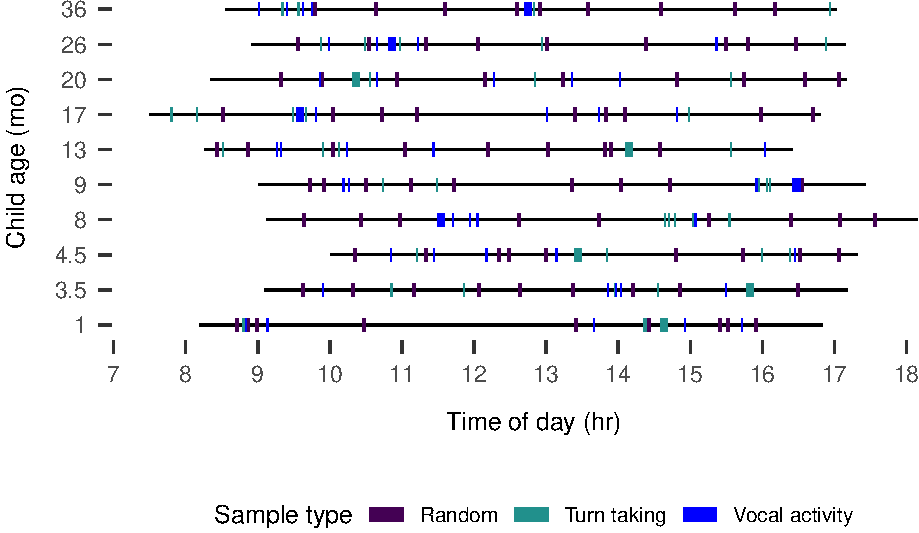
\includegraphics{Yeli-CLE_files/figure-latex/fig1-1.pdf}
\caption{\label{fig:fig1}Recording duration (black line) and sampled clips
(colored boxes) for each of the 10 recordings analyzed, sorted by child
age in months.}
\end{figure}

\subsection{Data selection and annotation}\label{methods-samples}

From the daylong recordings of XX Rossel children, we selected 10
representative children between ages 0;0 and 3;0 for transcription and
analysis in the current study. The 10 children were selected to be
spread between the target age range (0;0--3;0) while also representing a
range of typical maternal education levels found in the community and
being evenly split between male and female children
(\protect\hyperlink{tab1}{Table 1}; see also Bunce et al. (in
preparation)). For each child we then selected a series of
non-overalapping sub-clips from the day for transription
(\protect\hyperlink{fig1}{Figure 1}) in the following order: nine
randomly-selected 2.5-minute clips, five manually-selected
\enquote{peak} turn-taking activity 1-minute clips, five
manually-selected \enquote{peak} vocal activity 1-minute clips, and one
manually-selected 5-minute expansion of the best one-minute clip, for a
total of 37.5 minutes of transcribed audio for each child (6.25 audio
hours in total). The criteria for manual clip selection are identical to
those described for the parallel study on Tseltal by Casillas and
colleagues (forthcoming).

We were limited to selecting sub-clips from 10 children for analysis
because of the time-intensive nature of transcribing these naturalistic
data; 1 minute of audio typically took approximately 60--70 minutes to
be segmented into utterances, transcribed, annotated, and loosely
translated into English (\textasciitilde{}400 hours total). Given that
Yélî Dnye is nearly exclusively spoken on Rossel Island, where there is
no electricity and unreliable access to mobile data, transcription could
only be completed over the course of three 4--6 week visits by our
research group to the island in 2016, 2018, and 2019.

We used the ACLEW Annotation Scheme (Casillas et al., 2017a, 2017b) in
ELAN (Wittenburg, Brugman, Russel, Klassmann, \& Sloetjes, 2006) to
transcribe and annotate all hearable speech---both near and distant---in
the clips. We first segmented out the utterances and ascribed them to
individual speakers (e.g., older brother, mother, aunt, etc.). We then
annotated the vocal maturity of each utterance produced by the target
child (non-canonical babble/canonical babble/single
word/multi-word/unsure) and annotated the addressee of all speech from
other speakers (addressed to the target child/one or more other
children/one or more adults/a mix of adults and children/any
animal/other/unsure). Transcription and annotation was done together by
the first author and one of three community members (all native speakers
of Yélî Dnye). The community-based research assistants personally knew
all the families in the recordings, and were able to use their own
experience, the discourse context, and information from the accompanying
photos in reporting what was said and to whom speech was addressed for
each utterance. Detailed manuals and self-guided training materials,
including a \enquote{gold standard test} for this annotation scheme can
be found at \url{https://osf.io/b2jep/wiki/home/} (Casillas et al.,
2017b).

In what follows we first analyze the nine randomly selected 2.5-minute
clips from each child to establish a baseline view of their speech
environment, focusing on the effects of child age, time of day,
household size, and number of speakers on the rate of target
child-directed (TCDS) and other-directed speech (ODS). Next, we repeat
these analyses, focusing instead only on the turn-taking clips to gain a
view of the speech environment as it appears during the peak
interactions for the day. This latter set of analyses may more closely
mirror results from prior ethnographic work, which was designed to focus
on typical, lively interactions with young children. Then as a first
approximation of children's linguistic development, we map a coarse
trajectory of children's use of babble, first words, and multi-word
utterances. Finally, we wrap up by integrating our Panoramic-approach
results with those from prior Close Study work, relating these findings
to the larger literature on child-directed speech and its role in
language development.

\subsection{Statistical models}\label{statistical-models}

We conducted all analyses in R, using the glmmTMB package to run
generalized linear mixed-effects regressions on our dependent measures
(M. E. Brooks et al., 2017; R Core Team, 2018). We used ggplot2 to
generate all plots (Wickham, 2009). The dataset and scripts used in this
study can be found at \url{https://github.com/marisacasillas/Yeli-CLE}.
As in previous work on child speech environment measures (Bunce et al.,
in preparation; Casillas et al., forthcoming), TCDS and ODS minutes per
hour are naturally restricted to non-negative (0--infinity) values,
causing the distributional variance of those measures to become
positively skewed. To address this issue we use negative binomial
regressions, which can better fit non-negative, overdispersed data (M.
E. Brooks et al., 2017; Smithson \& Merkle, 2013). There were also many
cases of zero minutes of TCDS across the clips---for example, this often
occurred in the randomly sampled clips when the child was sleeping in a
quiet area. To handle this additional distributional characteristic of
the data, we added a zero-inflation model to TCDS analysis which, in
addition to the count model of TCDS (e.g., testing effects of age on the
input rate), creates a a binary model to evaluate the likelihood of TCDS
being used at all. More conventional, gaussian linear mixed-effects
regressions with log-transformed dependent variables are available in
the Supplementary Materials. The results of those alternative models are
qualitatively similar to what we report here.

\section{Results}\label{results}

The models included the following predictors: child age (months;
centered and standardized), household size (number of people; centered
and standardized), number of non-target-child speakers present in that
clip (centered and standardized), and time of day at the start of the
clip (factor: \enquote{morning} = before 11:00; \enquote{midday} =
11:00--13:00; \enquote{afternoon} = after 13:00). In addition, we
included two-way interactions: (a) child age and the number of speakers
present and (b) child age and time of day. We also added a random effect
of child. For the zero-inflation model of TCDS, we included the number
of speakers present. We limit our discussion here to significant effects
in the models; full model results, including gaussian alternative
models, are available in the Supplementary Materials.

\begin{figure}
\centering
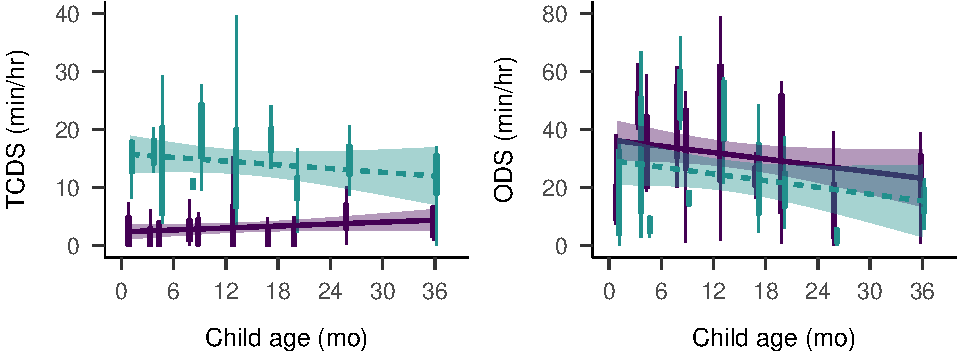
\includegraphics{Yeli-CLE_files/figure-latex/fig2-1.pdf}
\caption{\label{fig:fig2}Estimates of TCDS min/hr (left) and ODS min/hr
(right) across the sampled age range. Each box plot summarizes the data
for one child from the randomly sampled clips (purple; solid) or the
turn taking clips (green; dashed). Bands on the linear trends show 95\%
confidence intervals.}
\end{figure}

\subsection{Target-child-directed speech
(TCDS)}\label{target-child-directed-speech-tcds}

In the random sample, these 10 children heard an average of 3.13 minutes
of speech directly addressed to them per hour (median = 2.95; range =
1.58--6.26; \protect\hyperlink{fig2}{Figure 2}). For comparison, this is
slightly less than reported values using a near-identical method of data
collection, annotation, and analysis in a Tseltal Mayan community (3.6
minutes per hour for children under 3;0; Casillas et al., fortchoming)
and comparable to what has been reported using a similar method in a
Tsimane community (4.8 minutes per hour for children under 3;0 including
all hearable speech; 1.6 minutes when excluding overlap and far-away
speech; Scaff et al., in prep).

The zero-inflated negative binomial regression of TCDS minutes per hour
(N = 90, log-likelihood = -195.26, overdispersion estimate = 3.37)
suggested significant effects of child age, time of day, and their
interaction on the rate at which children hear speech addressed directly
to them. First, the older children heard significantly more TCDS per
hour (B = 0.73, SD = 0.23, z = 3.20, p \textless{} 0.01), with an
average increase of 0.73 minutes per hour for every month of
development. Overall, these children were also more likely to hear TCDS
in the mornings (see \protect\hyperlink{fig3}{Figure 3} for an overview
of time-of-day findings), with significantly higher TCDS rates in the
morning compared to both midday (B = 0.80, SD = 0.36, z = 2.23, p =
0.03) and the afternoon (B = 0.54, SD = 0.26, z = 2.10, p = 0.04), and
no significant difference in TCDS rate between midday and the afternoon.
However, the time-of-day pattern changed with child age. Older children
were more likely than younger children to show a peak in TCDS during
midday, with a decrease in TCDS between midday and the afternoon (B =
-0.60, SD = 0.29, z = -2.04, p = 0.04) and marginally less TCDS in the
morning than at midday (B = -0.59, SD = 0.30, z = -1.94, p = 0.05).
There were no other significant effects in either the count or the
zero-inflation model.

Children heard TCDS from a variety of different speakers. Overall, most
TCDS came from adults (mean = 72.65\%, median = 75.51\%, range =
41.41--100\%). On average, 82.35\% of the total adult TCDS minutes came
from women. That said, an increasing quantity of TCDS came from child
speakers (child-TCDS, e.g., from siblings and cousins;
\enquote{C-TCDS}); a Spearman's correlation showed a significant
positive relationship between the average proportion of C-TCDS in a clip
and target child age (Spearman's \emph{rho} = 0.78; \emph{p} = 0.01).

\begin{figure}
\centering
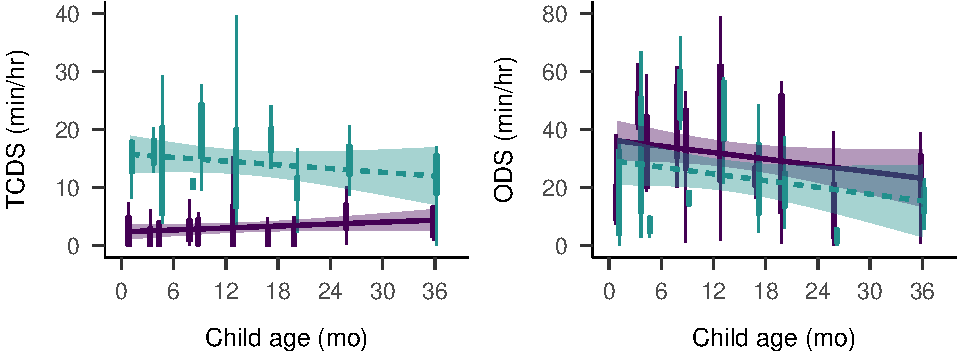
\includegraphics{Yeli-CLE_files/figure-latex/fig3-1.pdf}
\caption{\label{fig:fig3}Estimates of TCDS min/hr (left panels) and ODS
min/hr (right panels) across the recorded day in the random clips (top
panels) and turn-taking (bottom panels) clips. Each box plot summarizes
the data for children age 1;0 and younger (light) or age 1;0 and older
(dark) at the given time of day.}
\end{figure}

\subsection{Other-directed speech
(ODS)}\label{other-directed-speech-ods}

In the random sample, these children heard an average of 35.90 minutes
of other-directed speech per hour (median = 32.37; range =
20.20--53.78): that is more than eleven times the average quantity of
speech directed to them, with some children experiencing near-continuous
background speech. For comparison, a prior estimate for Tseltal Mayan
children using near-parallel methods to the present study found an
average of 21 minutes of overhearable speech per hour (Casillas et al.,
forthcoming), and a recent study of North American children's daylong
recordings found that adult-directed speech occurred at a rate of 7.3
minutes per hour (Bergelson et al., 2019).

The negative binomial regression of other-directed speech rate (N = 90,
log-likelihood = -370.87, overdispersion estimate = 9.14) revealed
effects of child age, number of speakers present, and time of day on the
rate of ODS encountered. The rate of ODS significantly decreased with
child age (B = -0.57, SD = 0.17, z = -3.28, p \textless{} 0.01) and
significantly increased in the presence of more speakers (B = 0.50, SD =
0.05, z = 10.07, p \textless{} 0.001). Across the randomly selected
clips, there were an average of 6.19 speakers present other than the
target child (median = 6; range = 1--19), an average of 59.99\% of whom
were adults. Comparing again to Tseltal and North American English, in
which the average number of speakers present was 3.44 and 3.9
respectively (Bergelson et al., 2019a; Casillas et al., forthcoming), we
can infer that the increased rate of ODS on Rossel Island is due in part
to there simply being more speakers present. Time-of-day effects on ODS
only came through in an interaction with child age. In particular, older
children heard a pattern of ODS mirroring the general pattern of TCDS;
significantly more ODS in the mornings compared to midday
(midday-vs-morning: B = 0.65, SD = 0.20, z = 3.23, p \textless{} 0.01)
and the afternoon (afternoon-vs-morning: B = 0.37, SD = 0.15, z = 2.50,
p = 0.01). There were no other significant effects on ODS rate in the
model.

In sum, the random baseline rates of TCDS and ODS in children's speech
environments are influenced by child age (TCDS increases, ODS
decreases), time of day (both generally peak in the morning), and their
interaction (older children hear more TCDS and less ODS at midday). The
rate of ODS is also impacted by the large number of speakers present in
some clips. Correlational results suggest that TCDS comes increasingly
from other children over the first three years. That said, the baseline
rate of TCDS is low, on par with estimates in other small-scale farming
communities (Casillas et al., forthcoming; Scaff et al., in prep); while
the ODS rate is quite high relative to estimates in prior work.

\subsection{TCDS and ODS during interactional
peaks}\label{tcds-and-ods-during-interactional-peaks}

If we instead investigate the rates of TCDS and ODS encountered by these
children during their interactional peaks for the day, a different
picture emerges (\protect\hyperlink{fig2}{Figures 2} and
\protect\hyperlink{fig3}{3} green/dashed summaries). In particular, the
children heard much more TCDS in the turn-taking clips---14.45 min/hr;
that is, more than four times the rate of TCDS in the random baseline
(median = 15.07; range = 9.61--18.73). During these same clips, children
heard a reduced rate of ODS: 25.27 min/hr (70.39\% of the random-sample
ODS rate; median = 19.59; range = 6.68--60.18). The negative binomial
mixed-effects regression of TCDS (N = 55, log-likelihood = -183.25,
overdispersion estimate = 2.91) revealed a significant decrease with
child age (B = -0.63, SD = 0.27, z = -2.33, p = 0.02) and a significant
interaction between child age and time of day; TCDS rate during
interactional peaks was marginally higher for older children at morning
compared to midday (midday-vs-morning: B = 0.53, SD = 0.28, z = 1.89, p
= 0.06) and significantly higher in the afternoon than at midday
(midday-vs-afternoon: B = 0.61, SD = 0.28, z = 2.17, p = 0.03).

As in the random sample, an increasing portion of TCDS during
interactional peaks came from other children. While, overall,
\emph{more} of the TCDS in interactional peaks came from adults than in
the random clips (mean = 82.68\%, median = 88.04\%, range = 50--100\%),
a Spearman's correlation showed an even stronger positive relationship
between the average proportion of child TCDS in a clip and target child
age (Spearman's \emph{rho} = 0.92; \emph{p} = \textless{} 0.001).
Notably, women contributed proportionally less TCDS during interactional
peaks than they did during the random clips: on average, women
contributed 61.55\% of the children's adult TCDS minutes in the
turn-taking clips (compared to 82.35\% in the random clips). In brief,
interactional peaks include more directed speech from men and more
directed speech from other children, with age.

The negative binomial mixed-effects regression of ODS (N = 55,
log-likelihood = -202.60, overdispersion estimate = 4.66) only revealed
a significant effect of number of speakers. As before, ODS rates were
higher when more speakers were present (B = 0.56, SD = 0.08, z = 6.76, p
\textless{} 0.001). There were no other significant effects on ODS rate
in the turn-taking clips.

Overall, the results suggest that these children typically hear very
little directly addressed speech, but that interactional peaks provide
opportunities for dense input at multiple points during the day. While
the majority of directed speech comes from women, an increasing portion
of it comes from other children with age, and directed speech from men
is more likely during interactional peaks. Directed and overhearable
speech is most likely to occur during the morning, before most of the
household has dispersed for their work activities, similar to other
findings from subsistence farming households (Casillas et al.,
forthcoming). However, older children are more likely than younger
children to show higher input rates at midday, perhaps due to their
increased interactions with other children while adults attend to
gardening and domestic tasks; we leave investigation of this idea to
future work. Possibly because of the large number of speakers typically
present, these children also experienced a high rate of overhearable
speech, underscoring the availability of other-addressed speech as a
resource for linguistic input in this context.

\subsection{Vocal maturity}\label{vocal-maturity}

Given the low overall rate of directed speech in these children's
environments, we might expect that their early linguistic development,
particularly the onset and use of single- and multi-word utterances, is
delayed in comparison to children growing up in more CDS-rich
environments. To briefly investigate this we plotted the proportion of
all linguistic vocalizations for each child (i.e., discarding laughter,
crying, or unknown-type vocalizations; leaving a total of 4308
vocalizations) that fell into the following categories: non-canonical
babble, canonical babble, single-word utterance, or multi-word
utterance. With development, children are expected to traverse all four
types of vocalization, such that they primarily produce single- and
multi-word utterances by age three.

In the onset of use for canonical babble, first words, and multi-word
utterances, these Rossel children's vocalization data closely resemble
expectations based on populations of children who hear more CDS
(\protect\hyperlink{fig4}{Figure 4}). That is, canonical babble appears
in the second half of the first year, first words appear around the
first birthday, and multi-word utterances appear a few months after that
(Frank, Braginsky, Marchman, \& Yurovsky, in preparation; Kuhl, 2004;
Pine \& Lieven, 1993; Slobin, 1970; Tomasello \& Brooks, 1999;
Warlaumont, Richards, Gilkerson, \& Oller, 2014). Notably, these
children also far exceed the usage rate of speech-like vocalizations
associated with major developmental delay. The canonical babbling ratio
(CBR; proportional use of speech-like vocalizations) associated with
developmental delay is 0.15 or below at age 0;10 or older. This 0.15
threshold is exceeded by all the Rossel children above 0;9, with a
minimum CBR of 0.22 at age 0;9 (mean = 0.63; median = 0.68; range =
0.22--0.86; see also Cychosz et al. (under reviewa)).

Over all annotated clips, children produced an average of 7.18
linguistic vocalizations per minute (median = 7.79; range = 4.57--8.95),
which is less than might be expected in American infant-caregiver
recordings (D. K. Oller, Eilers, Basinger, Steffens, \& Urbano, 1995).
However, this rate does align well with the frequency of child-initiated
prompts estimated for Rossel interaction in Close Study work (Brown,
2011). The rate also matches estimates for Tseltal Mayan children, who
hear a similar quantity of directed speech during this age range
(Casillas et al., forthcoming).

\begin{figure}
\centering
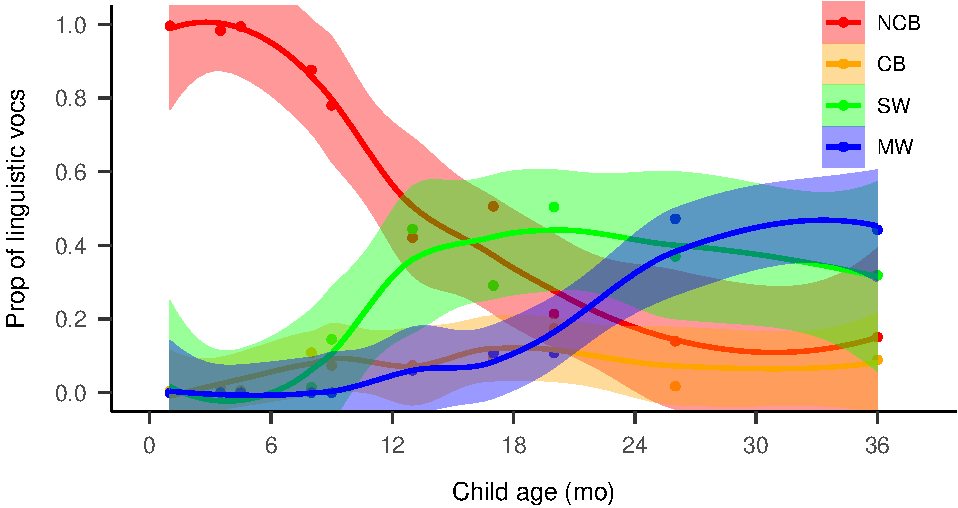
\includegraphics{Yeli-CLE_files/figure-latex/fig4-1.pdf}
\caption{\label{fig:fig4}Proportion of vocalization types used by children
across age (NCB = Non-canonical babble, CB = Canonical babble, SW =
single word utterance, MW = multi-word utterance).}
\end{figure}

\section{Discussion}\label{disc}

We analyzed the speech environments of 10 Rossel children under age 3;0
to investigate: (a) how often children were spoken to directly, (b) how
much other overhearable speech is available to them, (c) how these
sources of linguistic input are shaped by child age and interactional
context, and (d) whether this (relatively) low rate of directed input
appears to impact their early production milestones.

Based on prior ethnographic work, we expected that these children would
hear frequent child-directed speech from a wide variety of caregivers
and frequent speech directed to others (Brown \& Casillas, in press). In
fact children were rarely directly addressed. This low baseline rate of
TCDS is comparable---even slightly less---than that found in a Tseltal
Mayan community where minimal TCDS is one means to socializing children
into attending to their surroundings. On the other hand, the Rossel
child speech environment contains ample overhearable speech; much more
than has been reported in other communities at time of writing. We
suspect that both the low relative rate of TCDS and the high incidence
of ODS are partly attributable to the fact that multiple speakers are
typically present in the recordings, as discussed further below.

Prior work using similar methods to those presented here, also led us to
expect that the quantity of TCDS would be stable across the age range
studied (Bergelson et al., 2019b; Casillas et al., forthcoming; Scaff et
al., in preparation), and that an increasing proportion of it would come
from other children (Brown, 2011; Brown \& Casillas, in press; L. A.
Shneidman \& Goldin-Meadow, 2012). Counter to expectations, we found a
small but significant increase in TCDS rate with child age in the random
clips and a small but significant decrease in TCDS rate with age in the
turn-taking clips. The age-related baseline increase in TCDS may derive
from more frequent participation in independent play with other
children; in prior work, increased proportional input from other
children was also associated with an increase in overall input rate (L.
A. Shneidman \& Goldin-Meadow, 2012). The age-related decrease in TCDS
rate during peak interactional moments was not expected, but may be
attributable to this change in interactional partners with age; if
adults are more likely to be the source of TCDS during interactional
peaks for younger children, they may also provide more voluminous speech
during those peaks than other children do during interactional peaks
later in development. Both of these explanations require follow-up work
from a larger sample of children and, ideally, from a larger sample of
their interactions throughout the day. As expected based on prior
Panoramic work from both Western and non-Western samples (Bergelson et
al., 2019b; Casillas et al., forthcoming), we did see a decrease in ODS
with age.

Finally, while we anticipated that the children's input would be
non-uniformly distributed over the recording day (Abney et al., 2017;
Blasi et al., in preparation; Casillas et al., forthcoming), we also
expected to see a somewhat even distribution of directed speech from
morning to evening given that young Rossel children have been reported
to pass between multiple caregivers during a typical day at home. We
expected that this care-sharing practice might weaken the effect of
farming activities on linguistic input rate, found in the late morning
and early afternoon in previous work with Tseltal Mayan subsistence
farmers (Casillas et al., forthcoming). In fact, we found that
children's rate of linguistic input was still significantly impacted by
time of day, similar to prior work (Casillas et al., forthcoming). In
paricular, most TCDS and ODS came during the morning, with older
children more likely to hear TCDS at midday than younger children,
possibly because this is when most adults are likely attending to
gardening and domestic duties while children congregate in large play
groups.

\subsection{Diverging Close Study and Panoramic
perspectives}\label{diverging-close-study-and-panoramic-perspectives}

We predicted that infants on Rossel Island would hear more frequent
directed speech than has been found in other subsistence farming
contexts, like the Tseltal Mayan community discussed above (Brown, 2011,
2014; Brown \& Casillas, in press; Casillas et al., forthcoming). We
made this prediction on the basis of two prior ethnographic observations
(see Brown \& Casillas, in press for details). First, Rossel adults and
children have been shown to like \enquote{talking} to children, even
young infants, as if they can understand and respond to what is being
said. Second, infants and young children were observed to have access to
a wide network of caregivers who derive much joy from interacting with
them. Our Panoramic findings differ from these expectations: there is
minimal TCDS to young children, time of day strongly impacts the rate of
linguistic input, and there is limited variability in the type of
speakers typically talking to children.

We found that the 10 Rossel children here heard slightly less TCDS than
was documented for the Tseltal children. Taking the Mayan and Papuan
findings together, we suggest that the Panoramic approach is not
effective for distinguishing distinct caregiver approaches to talking to
young children. While Rossel caregivers view their children, even their
young infants, as potential co-interactants in conversational play
(Brown \& Casillas, in press), the circumstances of everyday life shape
the children's broader linguistic landscape such that most of what
children hear is talk between others. Specifically we suggest that, in
the daylong context, caregivers from these two subsistence farming
communities are preoccupied for most of the day with social and domestic
commitments in which they are motivated to converse with the other
adults and (older) children present; not just to get their daily tasks
done but also because these more mature speakers enable more complex
verbal interactions and social routines. Given the multi-generational
and patrilocal settlement patterns in both communities, there are
frequent opportunities to seek the company of other adults and older
children. This same explanation extends to the variability in linguistic
input encountered by children over the day and from different speaker
types; rather than being passed between caregivers who are
\enquote{free} to interact with them, young children may accompany their
varied caregivers in their shared daily tasks, switching from lap to lap
without the activity context changing.

When it comes to quantifying how much linguistic input children
encounter, the Panoramic view yields the important insight that direct
linguistic input is rare on average; it exists, but only during short
interactional peaks. We suspect that it is during these interactional
peaks, similar to what is typically captured in Close Study approaches,
that caregiver attitudes about how to engage children in interaction are
most clearly expressed. Indeed it is during these interactional peaks
when we see not only more TCDS but also TCDS from more diverse speaker
types. In contrast, the Panoramic data demonstrate how the number of
speakers present and the routines of everyday life strongly shape the
overall rate of linguistic input available in children's linguistic
environments. That is, the forces shaping the \emph{frequency} of Rossel
children's linguistic input are somewhat independent from the forces
shaping the \emph{format} of their linguistic input. This insight is
critical in trying to join cognitive and social models of children's
early language development. After all, children---particularly children
in contexts with minimal TCDS---may do most of their language learning
during these short bursts in the day when they are jointly attending to
language during interactions with others. If so, it would be more
effecient to aim our models of learning and annotation time at these
interactional peaks. Indeed, such a hybrid approach may be optimal for
accessing varied, ecologically valid, culturally distinct codes of
verbal interaction while also sketching a stable picture of early
language exposure specific those same communities (L. A. Shneidman,
2010; L. A. Shneidman \& Goldin-Meadow, 2012). Initial evidence for this
idea already comes from Bergelson and colleagues' (2019a) findings, in
which the most frequent nouns used were more similar across households
in the daylong samples than the video samples. Further cross-cultural
work on children's ability to learn from massed and disttributed (e.g.,
Schwab \& Lew-Williams, 2016), and direct and overhearable language use
(L. Shneidman, in preparation) is a critical route for further
investigation into how these sources of linguistic input may be
leveraged for language development.

\subsection{Independence and
child-TCDS}\label{independence-and-child-tcds}

The increase in TCDS from other children in this Rossel data recalls
findings from Shneidman and Goldin-Meadow (2012) in which Yucatec Mayan
children's directed speech rate increased enormously with age, primarily
due to increased input from other children. We saw a significant, but
much smaller overall increase in TCDS in these 10 Rossel children's
recordings, with an increasing proportion of that input coming from
children. Interestingly, a prior study using near-identical methods to
this one with a Tseltal Mayan community---culturally more similar to the
Yucatec community studied in Shneidman and Goldin-Meadow (2012)---found
no evidence for increased input from other children (Casillas et al.,
forthcoming). The lack of child TCDS in that study was attributed to the
observation that Tseltal Mayan children only begin to engage in
independent, extended play with older siblings and cousins after age
three, older than the sampled children in the study. In comparison,
prior ethnographic work on Rossel Island highlights independence as a
primary concern for parents of young children; from early toddlerhood
Rossel children are encouraged to choose how they dress, when and what
to eat, and who to visit (Brown \& Casillas, in press). The formation of
hamlets in a cluster around a shared open area, typically close to a
water source with a shallow area, further nurtures a sense of safe, free
space in which children can wander. These features of childhood on
Rossel Island support extended independent play with siblings and
cousins from an early age and may therefore explain the strongly
increasing presence of child TCDS in the present data. Further work,
combining the time of day effects and interlocutor effects found here
with ethnographic interview data, are needed to explore these ideas in
full. The consequence of this pattern for learning is that children's
linguistic input shifts in the first three years, with proportionally
more speech coming from less mature talkers; how this influences their
early production and comprehension patterns, particularly given the
minimal overall amount of TCDS, is an open question.

\subsection{Limitations}\label{limitations}

The present study used Panoramic methods to get a broader view of 10
Rossel children's linguistic landscapes, but was limited in both the
number of children represented and the number of annotated minutes
analyzed per child. The data presented here, though transcribed, were
only analyzed for superficial features of children's linguistic
environment: input rates of directed and overhearable speech and
children's overall vocal maturity. A Close Study approach is needed in
order to make semantically rich interpretations of what children are
saying and hearing or to delineate cross-cultural differences in the
\emph{format} of child-directed speech (sometimes called CDS
\enquote{quality} features). We note that the most promising long-term
approach for comparative developmental language research includes a
focus on within-community variation or cross-linguistic variation within
related languages (e.g., Pye, 2017; Weisleder \& Fernald, 2013); in
contrast, we limit ourselves here to comparing Rossel children's
language environment to findings from ethnolinguistically unrelated
communities. Importantly, the data presented here come from an evolving
corpus of Yélî Dnye developmental data; any reader interested in citing
descriptive features of the Rossel child language environment should
visit the following address for up-to-date estimates:
\url{https://middycasillas.shinyapps.io/Rossel_Child_Language_Environment/}.
The information on that linked page will include any new data,
annotations, and analyses added after the publication of this study.

\subsection{Conclusion}\label{disc-conclusion}

Using the Panoramic approach, we estimate that, on average, children on
Rossel Island under age 3;0 hear 3.13 minutes of directed speech per
hour, with an average of 14.45 minutes per hour during peak interactive
moments during the day. Most of the directed speech they hear comes from
adults, but older children hear more directed speech from other
children. There is also an average 35.90 minutes per hour of
overhearable speech children might be able to learn from. Older children
heard more directed speech and less overhearable speech than younger
children; though a far greater gain in ratio of directed-to-overhearable
speech is observable for all children in our sample within the peak
interactions for the day. Despite this relatively low rate of directed
speech, these children's vocal maturity appears on-track with norms for
typically developing children in multiple diverse populations (Cychosz
et al., under reviewa; Lee, Jhang, Relyea, Chen, \& Oller, 2018;
Warlaumont et al., 2014). Our findings diverged in several ways from
expectations developed on the basis of prior ethnographic work in this
community, including the frequency of child-directed talk, the diversity
of talkers, and the distribution of talk over the course of the day.
When considered together with data from a Mayan community, the findings
suggest that the Panoramic approach, while well suited to gathering
inclusive, ecologically valid estimates of how much linguistic input
children hear, is also far more sensitive to circumstantial variation
(e.g., the number of speakers present) than it is to established
ideological variation in how caregivers talk to children. For the
latter, a Close Study or hybrid approach is needed (e.g., analyzing
interactional peaks). Whether child language development is better
predicted by meaningful individual differences in average circumstantial
variation (e.g., Panoramic input quantity), ideologically-based
variation (e.g., Close Study input characteristics; attitudes toward
pedagogical talk), or something in-between is a question for future
work. Cross-cultural and cross-linguistic data will have a major role to
play in teasing out the causal factors at play in this larger issue
relating children's early linguistic experience to their later language
development.

\section{Acknowledgements}\label{acknowledgements}

The collection and annotation of these recordings was made possible by
Taakêmê Ńamono, Ndapw:éé Yidika, and Y:aaw:aa Pikuwa; with thanks also
to the PNG National Research Institute, and the Administration of Milne
Bay Province. We thank and acknowledge the participating families and
the Rossel community at large for their continuing support. We also
acknowledge support from the ACLEW project and thank Maartje Weenink for
her help with manual clip selection. This work is supported by a NWO
Veni Innovational Scheme grant (275-89-033) to MC and by an ERC Advanced
Grant (269484 INTERACT) to SCL. This paper was written using the papaja
library in RStudio (Aust \& Barth, 2018).

\newpage

\section{References}\label{refs}

\begingroup
\setlength{\parindent}{-0.5in} \setlength{\leftskip}{0.5in}

\hypertarget{refs}{}
\hypertarget{ref-abney2017time}{}
Abney, D. H., Smith, L. B., \& Yu, C. (2017). It's time: Quantifying the
relevant time scales for joint attention. In G. Gunzelmann, A. Howes, T.
Tenbrink, \& E. Davelaar (Eds.), \emph{Proceedings of the 39th Annual
Meeting of the Cognitive Science Society} (pp. 1489--1494). London, UK.

\hypertarget{ref-anderson2019modeling}{}
Anderson, H., \& Fausey, C. (2019). Modeling nonuniformities in infants'
everyday speech environments. presented at the biennial meeting of the
society for research on child development. baltimore, md.

\hypertarget{ref-R-papaja}{}
Aust, F., \& Barth, M. (2018). \emph{papaja: Create APA manuscripts with
R Markdown}. Retrieved from \url{https://github.com/crsh/papaja}

\hypertarget{ref-bergelson2019day}{}
Bergelson, E., Amatuni, A., Dailey, S., Koorathota, S., \& Tor, S.
(2019a). Day by day, hour by hour: Naturalistic language input to
infants. \emph{Developmental Science}, \emph{22}(1), e12715.
doi:\href{https://doi.org/10.1111/desc.12715}{10.1111/desc.12715}

\hypertarget{ref-bergelsoncasillas2019what}{}
Bergelson, E., Casillas, M., Soderstrom, M., Seidl, A., Warlaumont, A.
S., \& Amatuni, A. (2019b). What do North American babies hear? A
large-scale cross-corpus analysis. \emph{Developmental Science},
\emph{22}(1), e12724.
doi:\href{https://doi.org/10.1111/desc.12724}{10.1111/desc.12724}

\hypertarget{ref-blasiIPhuman}{}
Blasi, D., Schikowski, R., Moran, S., Pfeiler, B., \& Stoll, S. (in
preparation). Human communication is structured efficiently for first
language learners: Lexical spikes.

\hypertarget{ref-brooks2017modeling}{}
Brooks, M. E., Kristensen, K., van Benthem, K. J., Magnusson, A., Berg,
C. W., Nielsen, A., \ldots{} Bolker, B. M. (2017). Modeling
zero-inflated count data with glmmTMB. \emph{bioRxiv}.
doi:\href{https://doi.org/10.1101/132753}{10.1101/132753}

\hypertarget{ref-brown2011cultural}{}
Brown, P. (2011). The cultural organization of attention. In A. Duranti,
E. Ochs, \& and B. B. Schieffelin (Eds.), \emph{Handbook of Language
Socialization} (pp. 29--55). Malden, MA: Wiley-Blackwell.

\hypertarget{ref-brown2014interactional}{}
Brown, P. (2014). The interactional context of language learning in
Tzeltal. In I. Arnon, M. Casillas, C. Kurumada, \& B. Estigarribia
(Eds.), \emph{Language in interaction: Studies in honor of Eve V. Clark}
(pp. 51--82). Amsterdam, NL: John Benjamins.

\hypertarget{ref-brownIPchildrearing}{}
Brown, P., \& Casillas, M. (in press). Childrearing through social
interaction on Rossel Island, PNG. In A. J. Fentiman \& M. Goody (Eds.),
\emph{Esther Goody revisited: Exploring the legacy of an original
inter-disciplinarian} (pp. XX--XX). New York, NY: Berghahn.

\hypertarget{ref-bunceIPCDS}{}
Bunce, J., Soderstrom, M., Rosemberg, C., Bergelson, E., Rowland, C.,
Warlaumont, A. S., \& Casillas, M. (in preparation). Quantity of
child-directed speech heard in five language communities.

\hypertarget{ref-casillas2019stepbystep}{}
Casillas, M., \& Cristia, A. (2019). A step-by-step guide to collecting
and analyzing long-format speech environment (lfse) recordings.
\emph{Collabra: Psychology}, \emph{5}(1), 24.
doi:\href{https://doi.org/10.1525/collabra.209}{10.1525/collabra.209}

\hypertarget{ref-casillas2017workflow}{}
Casillas, M., Bergelson, E., Warlaumont, A. S., Cristia, A., Soderstrom,
M., VanDam, M., \& Sloetjes, H. (2017a). A new workflow for
semi-automatized annotations: Tests with long-form naturalistic
recordings of children's language environments. In F. Lacerda, D. House,
M. Heldner, J. Gustafson, S. Strömbergsson, \& M. Włodarczak (Eds.),
\emph{Proceedings of the 18th annual conference of the international
speech communication association (INTERSPEECH 2017)} (pp. 2098--2102).
Stockholm, Sweden.
doi:\href{https://doi.org/10.21437/Interspeech.2017-1418}{10.21437/Interspeech.2017-1418}

\hypertarget{ref-Casillas-HB}{}
Casillas, M., Brown, P., \& Levinson, S. C. (2017). Casillas HomeBank
corpus. doi:\href{https://doi.org/10.21415/T51X12}{10.21415/T51X12}

\hypertarget{ref-casillasFCearly}{}
Casillas, M., Brown, P., \& Levinson, S. C. (forthcoming). Early
language experience in a tseltal mayan village. \emph{Child
Development}, \emph{XX}(X), XX--XX.

\hypertarget{ref-casillas2017ACLEWDAS}{}
Casillas, M., Bunce, J., Soderstrom, M., Rosemberg, C., Migdalek, M.,
Alam, F., \ldots{} Garrison, H. (2017b). Introduction: The ACLEW DAS
template {[}training materials{]}. Retrieved from
\url{https://osf.io/aknjv/}

\hypertarget{ref-Cychosz-HB}{}
Cychosz, M. (2019). Cychosz HomeBank corpus.

\hypertarget{ref-cychoszURcanonical}{}
Cychosz, M., Cristia, A., Bergelson, E., Casillas, M., Baudet, G.,
Warlaumont, A. S., \ldots{} Seidl, A. (under reviewa). Canonical babble
development in a large-scale crosslinguistic corpus. Retrieved from
\url{https://osf.io/ca6qu/}

\hypertarget{ref-cychoszURlongform}{}
Cychosz, M., Romeo, R., Soderstrom, M., Scaff, C., Ganek, H., Cristia,
A., \ldots{} Weisleder, A. (under reviewb). Longform recordings of
everyday life: Ethics for best practices.

\hypertarget{ref-deleon2011language}{}
de León, L. (2011). Language socialization and multiparty participation
frameworks. In A. Duranti, E. Ochs, \& and B. B. Schieffelin (Eds.),
\emph{Handbook of Language Socialization} (pp. 81--111). Malden, MA:
Wiley-Blackwell.
doi:\href{https://doi.org/10.1002/9781444342901.ch4}{10.1002/9781444342901.ch4}

\hypertarget{ref-demuth2006word}{}
Demuth, K., Culbertson, J., \& Alter, J. (2006). Word-minimality,
epenthesis and coda licensing in the early acquisition of english.
\emph{Language and Speech}, \emph{49}(2), 137--173.

\hypertarget{ref-frankIPvariability}{}
Frank, M. C., Braginsky, M., Marchman, V. A., \& Yurovsky, D. (in
preparation). \emph{Variability and consistency in early language
learning: The Wordbank project}. Retrieved from
\url{https://langcog.github.io/wordbank-book/}

\hypertarget{ref-gaskins2000childrens}{}
Gaskins, S. (2000). Children's daily activities in a Mayan village: A
culturally grounded description. \emph{Cross-Cultural Research},
\emph{34}(4), 375--389.
doi:\href{https://doi.org/10.1177/106939710003400405}{10.1177/106939710003400405}

\hypertarget{ref-kuhl2004early}{}
Kuhl, P. K. (2004). Early language acquisition: Cracking the speech
code. \emph{Nature Reviews Neuroscience}, \emph{5}(11), 831.
doi:\href{https://doi.org/10.1038/nrn1533}{10.1038/nrn1533}

\hypertarget{ref-lee2018babbling}{}
Lee, C.-C., Jhang, Y., Relyea, G., Chen, L.-m., \& Oller, D. K. (2018).
Babbling development as seen in canonical babbling ratios: A
naturalistic evaluation of all-day recordings. \emph{Infant Behavior and
Development}, \emph{50}, 140--153.

\hypertarget{ref-ochs1984language}{}
Ochs, E., \& Schieffelin, B. (1984). Language acquisition and
socialization: Three developmental stories and their implications. In R.
A. Schweder \& R. A. LeVine (Eds.), \emph{Culture theory: Essays on
mind, self, and emotion} (pp. 276--322). Cambridge University Press.

\hypertarget{ref-oller1995extreme}{}
Oller, D. K., Eilers, R. E., Basinger, D., Steffens, M. L., \& Urbano,
R. (1995). Extreme poverty and the development of precursors to the
speech capacity. \emph{First Language}, \emph{15}(44), 167--187.

\hypertarget{ref-pine1993reanalysing}{}
Pine, J. M., \& Lieven, E. V. M. (1993). Reanalysing rote-learned
phrases: Individual differences in the transition to multi-word speech.
\emph{Journal of Child Language}, \emph{20}(3), 551--571.
doi:\href{https://doi.org/10.1017/S0305000900008473}{10.1017/S0305000900008473}

\hypertarget{ref-pye1986quiche}{}
Pye, C. (1986). Quiché Mayan speech to children. \emph{Journal of Child
Language}, \emph{13}(1), 85--100.
doi:\href{https://doi.org/10.1017/S0305000900000313}{10.1017/S0305000900000313}

\hypertarget{ref-pye2017comparative}{}
Pye, C. (2017). \emph{The Comparative Method of Language Acquisition
Research}. University of Chicago Press.

\hypertarget{ref-R-base}{}
R Core Team. (2018). \emph{R: A language and environment for statistical
computing}. Vienna, Austria: R Foundation for Statistical Computing.
Retrieved from \url{https://www.R-project.org/}

\hypertarget{ref-rogoff2003firsthand}{}
Rogoff, B., Paradise, R., Arauz, R. M., Correa-Chávez, M., \& Angelillo,
C. (2003). Firsthand learning through intent participation. \emph{Annual
Review of Psychology}, \emph{54}(1), 175--203.
doi:\href{https://doi.org/10.1146/annurev.psych.54.101601.145118}{10.1146/annurev.psych.54.101601.145118}

\hypertarget{ref-scaffIPlanguage}{}
Scaff, C., Stieglitz, J., Casillas, M., \& Cristia, A. (in preparation).
Language input in a hunter-forager population: Estimations from daylong
recordings.

\hypertarget{ref-schwab2016repetition}{}
Schwab, J. F., \& Lew-Williams, C. (2016). Repetition across successive
sentences facilitates young children's word learning.
\emph{Developmental Psychology}, \emph{52}(6), 879--886.
doi:\href{https://doi.org/10.1037/dev0000125}{10.1037/dev0000125}

\hypertarget{ref-shneidmanIPoverhearing}{}
Shneidman, L. (in preparation). Learning from overhearind.

\hypertarget{ref-shneidman2010language}{}
Shneidman, L. A. (2010). \emph{Language Input and Acquisition in a Mayan
Village} (PhD thesis). The University of Chicago.

\hypertarget{ref-shneidman2012language}{}
Shneidman, L. A., \& Goldin-Meadow, S. (2012). Language input and
acquisition in a Mayan village: How important is directed speech?
\emph{Developmental Science}, \emph{15}(5), 659--673.
doi:\href{https://doi.org/10.1111/j.1467-7687.2012.01168.x}{10.1111/j.1467-7687.2012.01168.x}

\hypertarget{ref-slobin1970universals}{}
Slobin, D. I. (1970). Universals of grammatical development in children.
In G. B. Flores d'Arcais \& W. J. M. Levelt (Eds.), \emph{Advances in
Psycholinguistics} (pp. 174--186). Amsterdam, NL: North Holland
Publishing.

\hypertarget{ref-smithson2013generalized}{}
Smithson, M., \& Merkle, E. (2013). \emph{Generalized linear models for
categorical and continuous limited dependent variables}. New York:
Chapman; Hall/CRC.
doi:\href{https://doi.org/10.1201/b15694}{10.1201/b15694}

\hypertarget{ref-tamislemonda2017power}{}
Tamis-LeMonda, C. S., Kuchirko, Y., Luo, R., Escobar, K., \& Bornstein,
M. H. (2017). Power in methods: Language to infants in structured and
naturalistic contexts. \emph{Developmental Science}, \emph{20}(6),
e12456.
doi:\href{https://doi.org/10.1111/desc.12456}{10.1111/desc.12456}

\hypertarget{ref-tomasello1999early}{}
Tomasello, M., \& Brooks, P. J. (1999). Early syntactic development: A
Construction Grammar approach. In M. Barrett (Ed.), \emph{The
Development of Language} (pp. 161--190). New York: Psychology Press.

\hypertarget{ref-warlaumont2014social}{}
Warlaumont, A. S., Richards, J. A., Gilkerson, J., \& Oller, D. K.
(2014). A social feedback loop for speech development and its reduction
in Autism. \emph{Psychological Science}, \emph{25}(7), 1314--1324.
doi:\href{https://doi.org/10.1177/0956797614531023}{10.1177/0956797614531023}

\hypertarget{ref-weisleder2013talking}{}
Weisleder, A., \& Fernald, A. (2013). Talking to children matters: Early
language experience strengthens processing and builds vocabulary.
\emph{Psychological Science}, \emph{24}(11), 2143--2152.
doi:\href{https://doi.org/10.1177/0956797613488145}{10.1177/0956797613488145}

\hypertarget{ref-R-ggplot2}{}
Wickham, H. (2009). \emph{Ggplot2: Elegant graphics for data analysis}.
Springer-Verlag New York. Retrieved from \url{http://ggplot2.org}

\hypertarget{ref-ELAN}{}
Wittenburg, P., Brugman, H., Russel, A., Klassmann, A., \& Sloetjes, H.
(2006). ELAN: A professional framework for multimodality research. In
\emph{Proceedings of the Fifth International Conference on Language
Resources and Evaluation} (pp. 1556--1559).

\hypertarget{ref-xu2009reliability}{}
Xu, D., Yapanel, U., \& Gray, S. (2009). LENA tr-05: Reliability of the
lena language environment analysis system in young children's natural
language home environment. Boulder, CO: LENA Foundation.

\endgroup


\end{document}
